%texexptitled======================================================================
% lab1-gcd
%-----------------------------------------------------------------------
%

\documentclass[11pt]{article}

% Package includes

\usepackage{graphicx}
\usepackage{color}
\usepackage{comment}
\usepackage{multirow}
\usepackage{askmaps}
\usepackage{amssymb}
\usepackage{amsmath}
\usepackage{tikz}
\usepackage{circuitikzgit}
\usetikzlibrary{arrows, positioning, shapes.geometric, circuits.logic.US}
\tikzstyle{line}=[draw]
\tikzstyle{arrow}=[draw, -latex]

% Wrap long URLs with hyphens
\PassOptionsToPackage{hyphens}{url}\usepackage{hyperref}
\usepackage{pdftexcmds}
\usepackage{upquote}
\usepackage{textcomp}
\usepackage{minted}
\usepackage[listings]{tcolorbox}
\usepackage{enumerate}
\usepackage{enumitem}
\usepackage{mathtools}
\DeclarePairedDelimiter{\ceil}{\Big\lceil}{\Big\rceil}

\tcbset{
texexp/.style={colframe=black, colback=lightgray!15,
         coltitle=white,
         fonttitle=\small\sffamily\bfseries, fontupper=\small, fontlower=\small},
     example/.style 2 args={texexp,
title={Question \thetcbcounter: #1},label={#2}},
}

\newtcolorbox{texexp}[1]{texexp}
\newtcolorbox[auto counter]{texexptitled}[3][]{%
example={#2}{#3},#1}

\setlength{\topmargin}{-0.5in}
\setlength{\textheight}{9in}
\setlength{\oddsidemargin}{0in}
\setlength{\evensidemargin}{0in}
\setlength{\textwidth}{6.5in}

% Useful macros

\newcommand{\note}[1]{{\bf [ NOTE: #1 ]}}
\newcommand{\fixme}[1]{{\bf [ FIXME: #1 ]}}
\newcommand{\wunits}[2]{\mbox{#1\,#2}}
\newcommand{\um}{\mbox{$\mu$m}}
\newcommand{\xum}[1]{\wunits{#1}{\um}}
\newcommand{\by}[2]{\mbox{#1$\times$#2}}
\newcommand{\byby}[3]{\mbox{#1$\times$#2$\times$#3}}


\newenvironment{tightlist}
{\begin{itemize}
 \setlength{\parsep}{0pt}
 \setlength{\itemsep}{-2pt}}
{\end{itemize}}

\newenvironment{titledtightlist}[1]
{\noindent
 ~~\textbf{#1}
 \begin{itemize}
 \setlength{\parsep}{0pt}
 \setlength{\itemsep}{-2pt}}
{\end{itemize}}

% Change spacing before and after section headers

\makeatletter
\renewcommand{\section}
{\@startsection {section}{1}{0pt}
 {-2ex}
 {1ex}
 {\bfseries\Large}}
\makeatother

\makeatletter
\renewcommand{\subsection}
{\@startsection {subsection}{1}{0pt}
 {-1ex}
 {0.5ex}
 {\bfseries\normalsize}}
\makeatother

% Reduce likelihood of a single line at the top/bottom of page

\clubpenalty=2000
\widowpenalty=2000

% Other commands and parameters

\pagestyle{myheadings}
\setlength{\parindent}{0in}
\setlength{\parskip}{10pt}

% Commands for register format figures.

\newcommand{\instbit}[1]{\mbox{\scriptsize #1}}
\newcommand{\instbitrange}[2]{\instbit{#1} \hfill \instbit{#2}}

\newif\ifsolution

\if\issolution1
\newenvironment{solution}
    {\color{red}}
    {\color{black}}
\solutiontrue
\else
\excludecomment{solution}
\solutionfalse
\fi


\graphicspath{{./figs/}}


%-----------------------------------------------------------------------
% Document
%-----------------------------------------------------------------------

\begin{document}
\def\PYZsq{\textquotesingle}


\newcommand{\headertext}{EE142 Problem Set 10}
\renewcommand{\thesubsection}{\thesection.\alph{subsection}}

\title{\vspace{-0.4in}\Large \bf \headertext \vspace{-0.1in}}
\author{Vighnesh Iyer}

\date{\today}
\maketitle

\markboth{\headertext}{\headertext}
\thispagestyle{empty}

\section{Mixer Analysis}
\begin{figure}[H]
    \centering 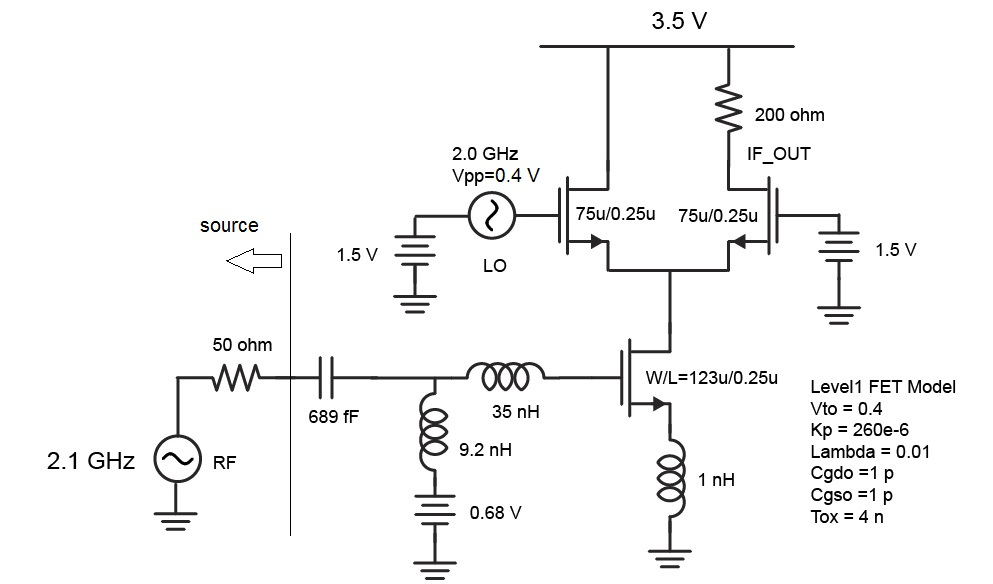
\includegraphics[width=1.0\textwidth]{problem1_schematic.jpg}
\end{figure}

\begin{enumerate}[label=(\alph*)]
    \item {\color{blue} For the FET mixer shown above with the FET parameters annotated, estimate (calculate) the mixer down-conversion power gain for an input RF signal at 2.1 GHz and LO at 2 GHz. Verify your estimation by ADS simulation.}

    We do the hand-calculations assuming a long-channel device.

    \begin{align*}
        I_d &= \frac{1}{2} K_p \frac{W}{L} (V_{gs} - V_{th})^2 \\
        &= 5 \text{ mA} \\
        g_m &= \frac{2 I_d}{V_{ov}} = 0.036 \\
        G_m &= Q \cdot g_m = 2.002 \cdot g_m = 0.072 \\
        I_{tail} &= I_d + v_s \cos(\omega_{RF} t) \cdot G_m \\
        &= 5 \text{ mA} + v_s \cos(\omega_{RF} t) \cdot 0.076 \\
        K &= \frac{1}{2} K_p \frac{W}{L} \\
        i_{d,1,2,diffpair} &\approx \frac{I_{tail}}{2} \pm \sqrt{2 K I_{tail}} \frac{v_{id}}{2} \text{ from disc slides} \\
        &= \frac{I_{tail}}{2} + \sqrt{2 K I_{dc}} (1 + \frac{I_{ac}}{2 I_{dc}}) \frac{v_{id}}{2} \\
        i_{IF} &= \sqrt{2 K I_{dc}} v_s \frac{G_m}{2 I_{dc}} \frac{0.2}{4} = 0.007 v_s \\
        v_{IF} &= 200 \cdot i_{IF} = 1.414 v_s
    \end{align*}

    The voltage conversion gain is 1.414.

    The ADS schematic:
    \begin{figure}[H]
        \centering 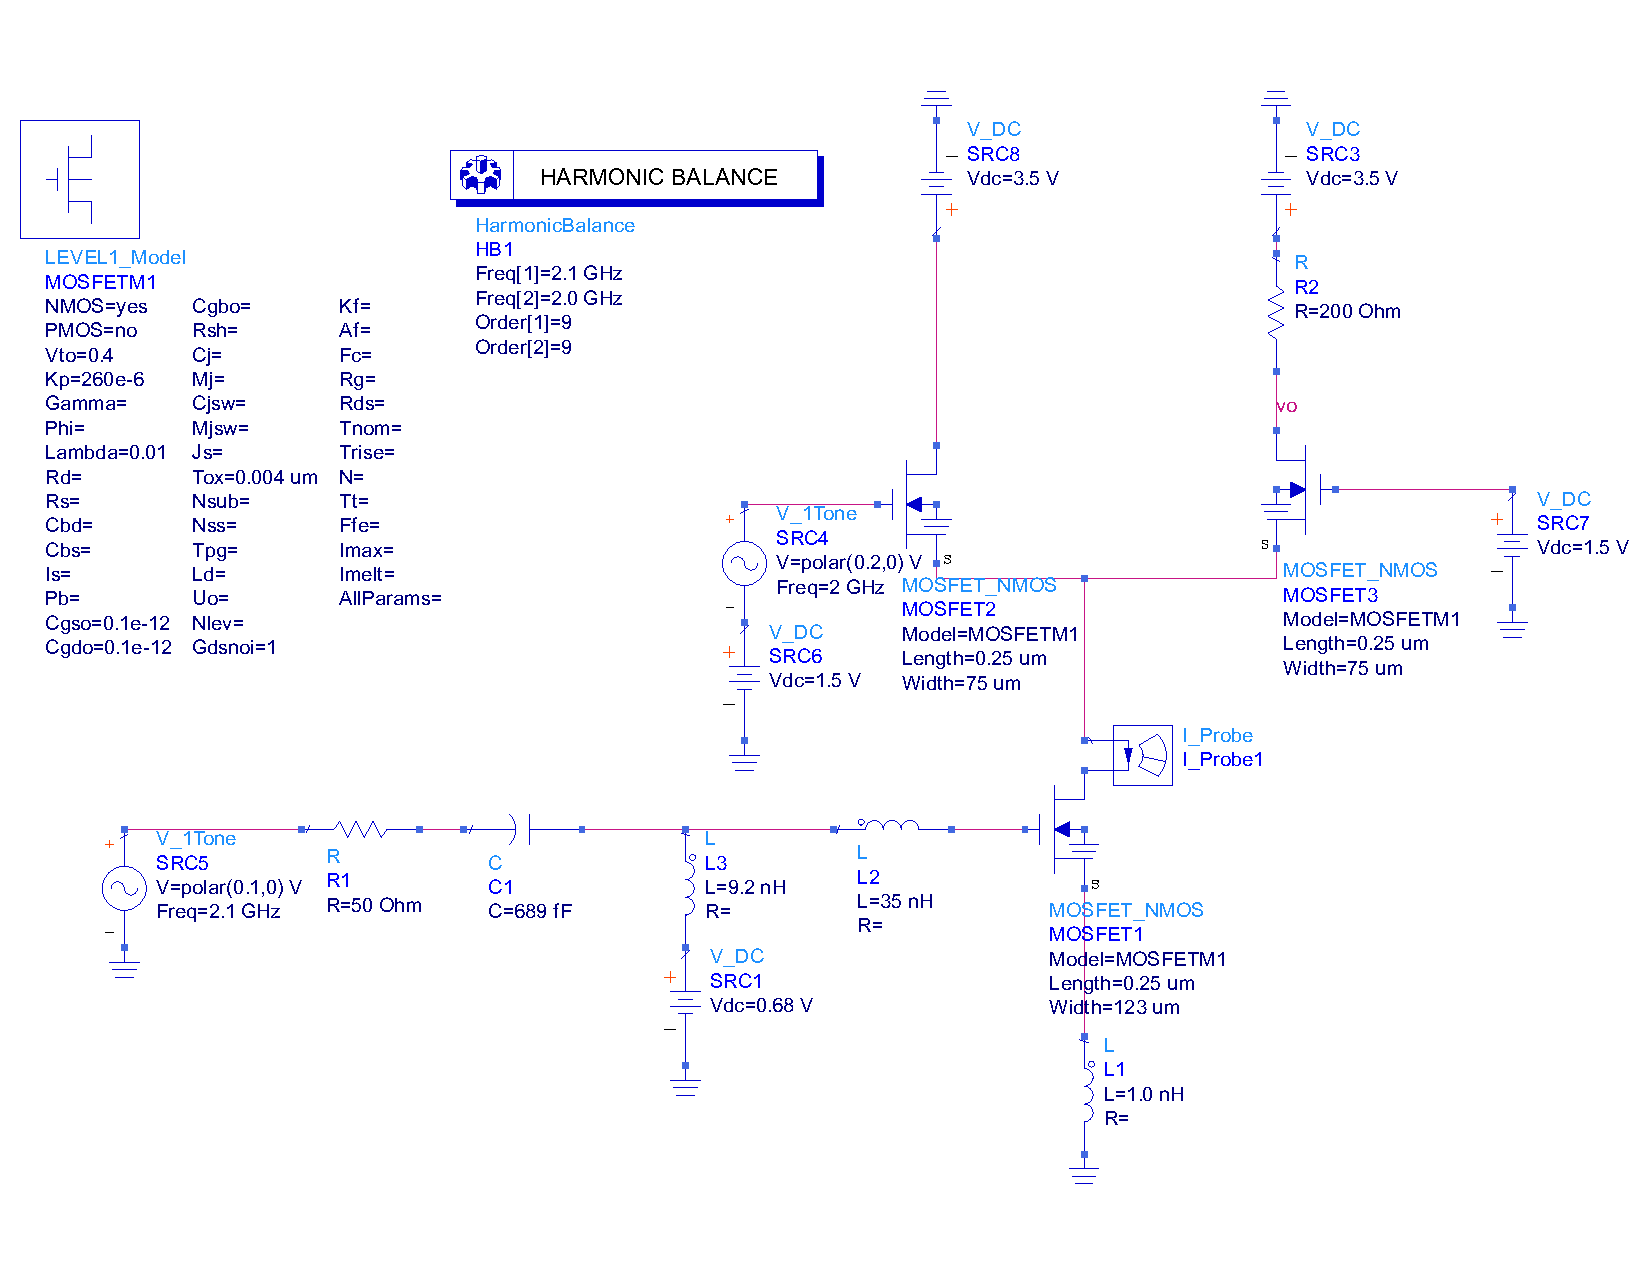
\includegraphics[width=0.8\textwidth]{problem1ab_schematic.pdf}
    \end{figure}

    Simulation results:
    \begin{figure}[H]
        \centering 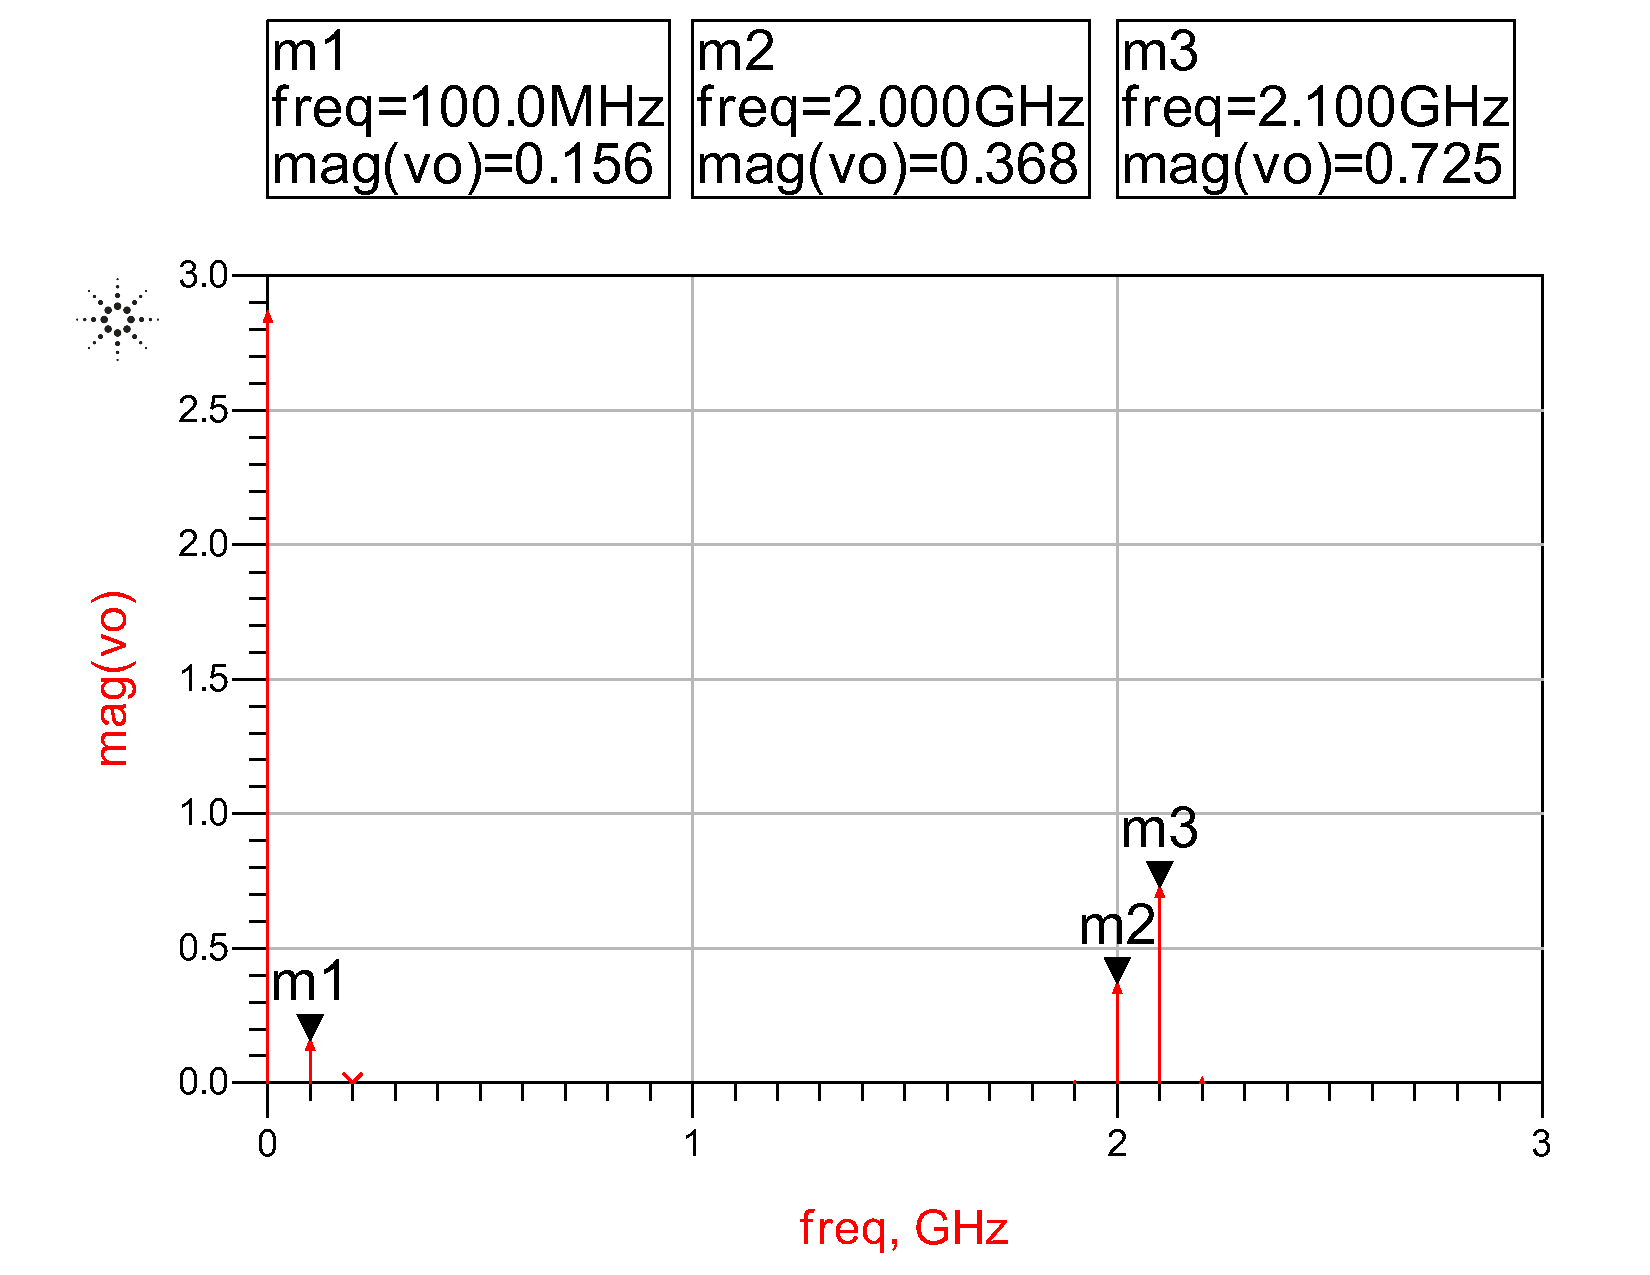
\includegraphics[width=0.5\textwidth]{problem1ab_sim_results.pdf}
    \end{figure}

    \item {\color{blue} Calculate the LO and RF leakages at the IF port. Verify your results by ADS simulation.}

    The RF-to-IF leakage is caused by the Q-boosted transconductance of the tail FET which flows through the IF FET.
    \begin{align*}
        v_{out,RF} = v_s G_m \frac{1}{2} \cdot 200 = 7.17 v_s
    \end{align*}

    The LO-to-IF leakage is caused by the differential swing on the IF FET.
    \begin{align*}
        v_{out,LO} = \sqrt{2 K I_{dc}} \frac{v_{id}}{2} \cdot R_L = 0.395 \text{ V}
    \end{align*}

    The simulation results closely match the hand calculation.

    \item {\color{blue} Simulate the mixer IIP3.}
    The ADS schematic:
    \begin{figure}[H]
        \centering 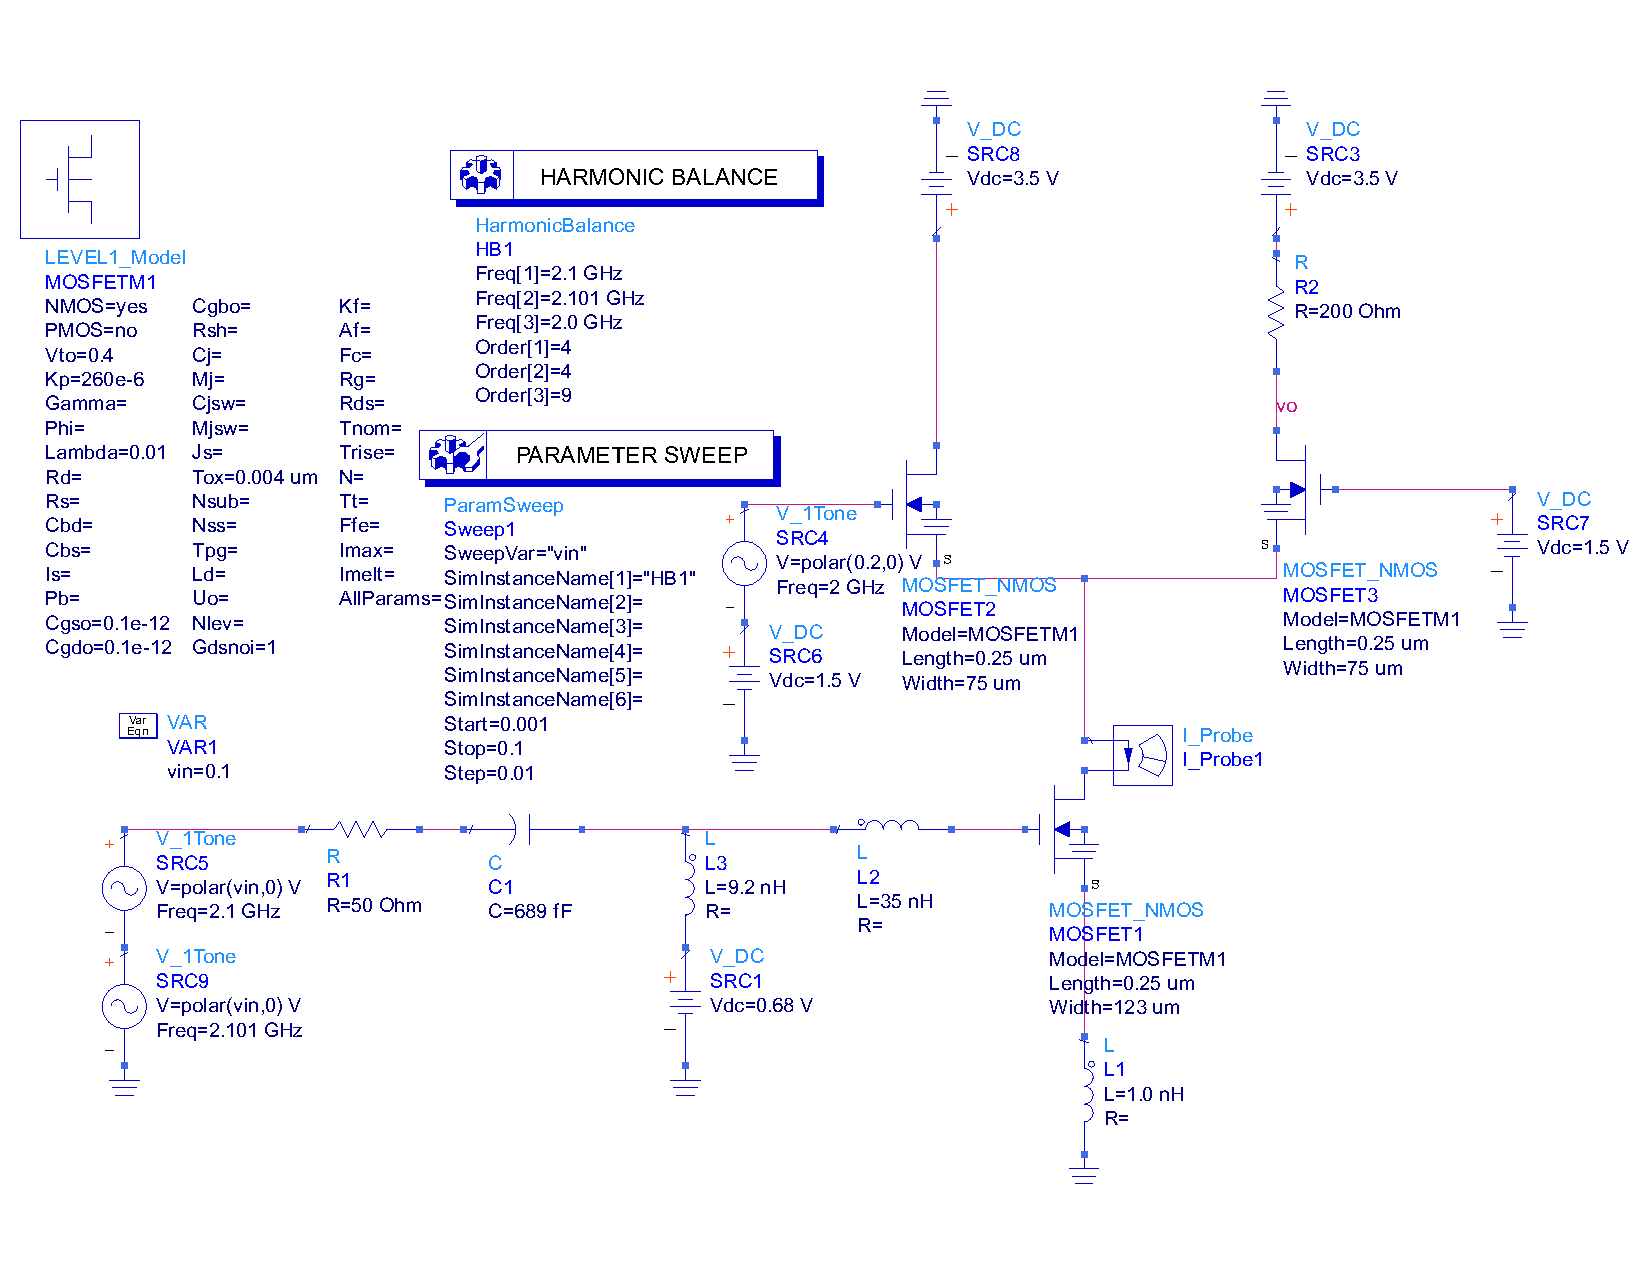
\includegraphics[width=0.8\textwidth]{problem1c_schematic.pdf}
    \end{figure}

    Simulation results:
    \begin{figure}[H]
        \centering 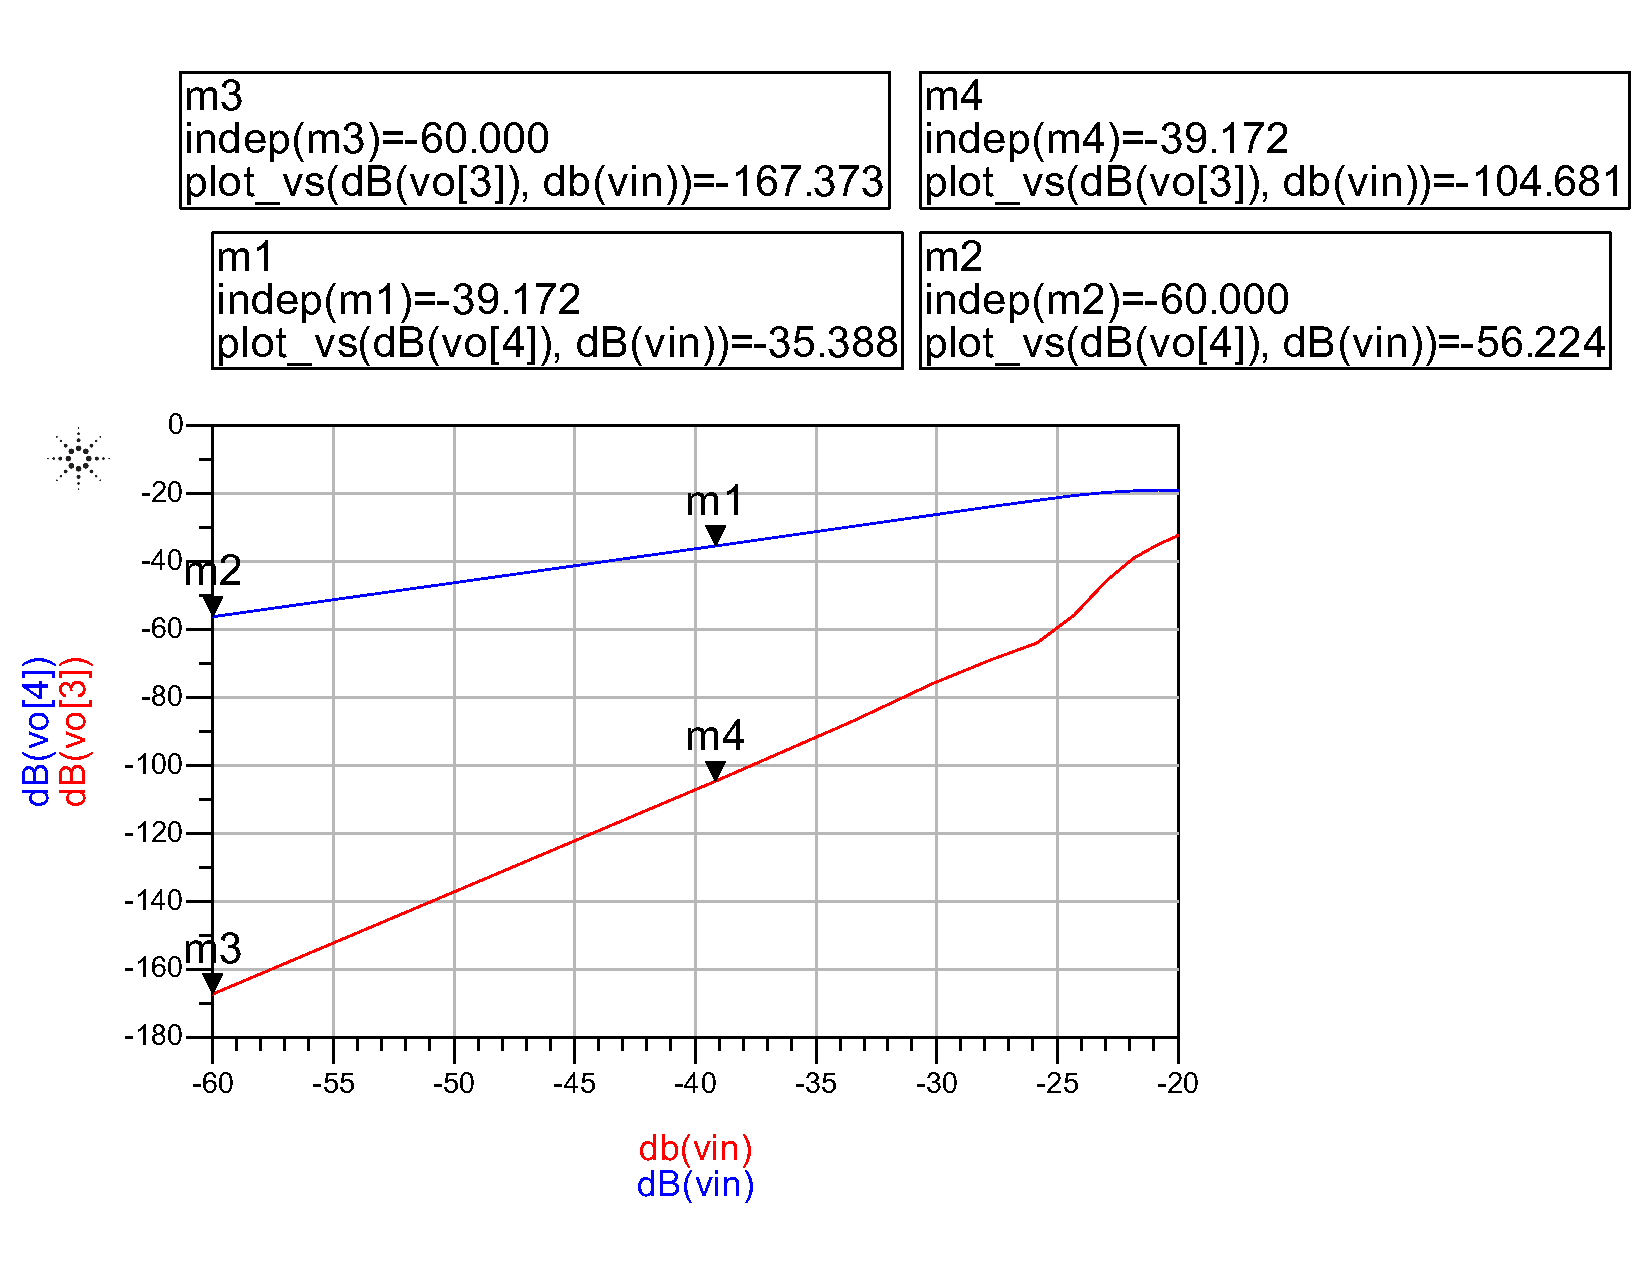
\includegraphics[width=0.6\textwidth]{problem1c_sim_results.pdf}
    \end{figure}

    We find that the extrapolated lines intersect at -4.69 dBV.

    \item {\color{blue} Estimate the mixer IIP3 by hand calculation.}
    Unfortunately, I don't have time to look into this part.

    \item {\color{blue} Repeat part (a) to part (c) with the LO drive enhanced to 0.8$V_{pp}$.}

    \item {\color{blue} Roughly estimate the mixer SSB NF. The noise of the FETs and the noise of the load resistance can be excluded. Use an LO drive of 0.4$V_{pp}$.}
\end{enumerate}

\section{Power Amplifier (PA) Output Waveform and Efficiency}
{\color{blue} Assume your FET transistor device has the following properties:
\begin{itemize}
    \item Maximum drain current of $I_{d,max}$
    \item Maximum drain voltage of $V_{d,max}$
    \item Minimum drain voltage of $V_{d,min}$
    \item If $V_g > 0.5$ then $I_d = (V_g - 0.5)$ else $I_d = 0$
    \item Input impedance of $50 \Omega$
\end{itemize}}

\begin{enumerate}[label=(\alph*)]
    \item {\color{blue} Design the transistor drain bias voltage, gate bias voltage, drain bias current, and load impedance (including the load impedance at harmonics of the operation frequency) for Class-A and Class-B power amplifier operations.}

    \item {\color{blue} What are the power gains of the two designs?}

    \item {\color{blue} Following part(a), draw the time-domain transistor voltage and current waveforms at the peak output for the two designs.}

    \item {\color{blue} Following part(a), draw the power delivered to the load, dc power consumption, and the drain efficiency for your Class-A and Class-B designs. The x-axis in your plots should be the input power back-off from the input level corresponding to the maximum output power.}

    \item {\color{blue} Following part(a), what are the peak power-added efficiencies (PAE) of your Class-A and Class-B PA designs?}
\end{enumerate}

\end{document}
